\documentclass{article}
\usepackage{tikz}
\usetikzlibrary{arrows.meta}

\begin{document}

\begin{figure}[h]
    \centering
    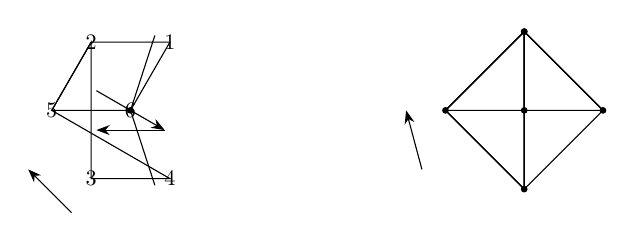
\begin{tikzpicture}[scale=1, every node/.style={scale=0.8}]

        % Drawing the graph on the left
        \draw (0,0) -- ++(72:1);
        \draw (0,0) -- ++(-72:1);
        \filldraw[black] (0,0) circle (1pt);
        \draw[->, >=Stealth] (-30:0.5) -- (210:0.5);
        \draw[->, >=Stealth] (150:0.5) -- (330:0.5);

        % Drawing the main diamond in the middle
        \coordinate (a) at (0,0);
        \coordinate (b) at (60:1);
        \coordinate (c) at (120:1);
        \coordinate (d) at (180:1);
        \coordinate (e) at (240:1);
        \coordinate (f) at (300:1);

        \draw (a) -- (b) -- (c) -- (d) -- cycle;
        \draw (c) -- (e) -- (f) -- (d) -- cycle;

        \node at (b) {$1$};
        \node at (c) {$2$};
        \node at (e) {$3$};
        \node at (f) {$4$};
        \node at (d) {$5$};
        \node at (a) {$6$};

        % Drawing the arrow pointing to the right
        \draw[->, >=Stealth] (240:1.5) -- (210:1.5);

        % Drawing the graph on the right
        \begin{scope}[shift={(5,0)}, rotate=90]
            \coordinate (g) at (0,0);
            \coordinate (h) at (0:1);
            \coordinate (i) at (90:1);
            \coordinate (j) at (180:1);
            \coordinate (k) at (270:1);
            \coordinate (l) at (360:1);
            \draw (g) -- (h) -- (i) -- (j) -- (k) -- (l) -- cycle;
            \draw (k) -- (l) -- (j) -- (h) -- cycle;
            \draw (h) -- (i) -- (j) -- (l) -- cycle;
            \draw (j) -- (l) -- (k) -- (i) -- cycle;
            \draw (i) -- (l) -- (k) -- (h) -- cycle;
            \draw (k) -- (l) -- (i) -- (h) -- cycle;
            \filldraw[black] (g) circle (1pt);
            \filldraw[black] (h) circle (1pt);
            \filldraw[black] (i) circle (1pt);
            \filldraw[black] (j) circle (1pt);
            \filldraw[black] (k) circle (1pt);
            \filldraw[black] (l) circle (1pt);
            \draw[->, >=Stealth] (120:1.5) -- (90:1.5);
        \end{scope}

    \end{tikzpicture}
    \caption{Figure of a symmetric replacement rule that produces the ``Laakso diamond'' space, as described in~\cite{Laakso, Yair, LangPlaut}.}
\end{figure}

\end{document}